%%%%%%%%%%%%%%%%%%%%%%%%%%%%%%%%%%%%%%%%%%%%%%%%%%%%%%%%%%%%%%%%%%%%%
% LaTeX Template: Project Titlepage Modified (v 0.1) by rcx
%
% Original Source: http://www.howtotex.com
% Date: February 2014
% 
% This is a title page template which be used for articles & reports.
% 
% This is the modified version of the original Latex template from
% aforementioned website.
% 
%%%%%%%%%%%%%%%%%%%%%%%%%%%%%%%%%%%%%%%%%%%%%%%%%%%%%%%%%%%%%%%%%%%%%%

\documentclass[12pt]{report}
\usepackage[a4paper]{geometry}
\usepackage[myheadings]{fullpage}
\usepackage{fancyhdr}
\usepackage{lastpage}
\usepackage{graphicx, wrapfig, subcaption, setspace, booktabs}
\usepackage[T1]{fontenc}
\usepackage[font=small, labelfont=bf]{caption}
\usepackage{fourier}
\usepackage[protrusion=true, expansion=true]{microtype}
\usepackage[english]{babel}
\usepackage{sectsty}
\usepackage{url}
\usepackage{listings}
\usepackage{color}
\usepackage{xcolor}

\newcommand{\HRule}[1]{\rule{\linewidth}{#1}}
\onehalfspacing
\setcounter{tocdepth}{5}
\setcounter{secnumdepth}{5}

\definecolor{dkgreen}{rgb}{0,0.6,0}
\definecolor{gray}{rgb}{0.5,0.5,0.5}
\lstset { 
language=C++,
backgroundcolor=\color{black!5}, % set backgroundcolor
basicstyle=\footnotesize,% basic font setting
}
%-------------------------------------------------------------------------------
% HEADER & FOOTER
%-------------------------------------------------------------------------------
\pagestyle{fancy}
\fancyhf{}
\setlength\headheight{15pt}
\fancyhead[L]{FlatB}
\fancyhead[R]{Programming Manual}
\fancyfoot[R]{Page \thepage\ of \pageref{LastPage}}
%-------------------------------------------------------------------------------
% TITLE PAGE
%-------------------------------------------------------------------------------

\begin{document}

\title{ \normalsize \textsc{Manual}
		\\ [2.0cm]
		\HRule{0.5pt} \\
		\LARGE \textbf{\uppercase{BFlat}}
		\HRule{2pt} \\ [0.5cm]
		\normalsize \today \vspace*{5\baselineskip}}

\date{}

\author{ Adarsh Sanjeev }

\maketitle
\tableofcontents
\newpage

%-------------------------------------------------------------------------------
% Section title formatting
\sectionfont{\scshape}
%-------------------------------------------------------------------------------

%-------------------------------------------------------------------------------
% BODY
%-------------------------------------------------------------------------------

\section*{Introduction}
\addcontentsline{toc}{section}{Introduction}
BFlat is a programming language

\section*{Syntax}
\addcontentsline{toc}{section}{Syntax}

This is syntax.

\subsection*{Datatypes}
\addcontentsline{toc}{subsection}{Datatypes}

FlatB only has integers as valid datatypes for variables. However, strings are allowed as string literals for use in print statements.
The variables can be of array datatype also.

\subsection*{Statements}
\addcontentsline{toc}{subsection}{Statements}
Each statement in FlatB must end with a semicolon and be of one of the following types.

\subsubsection*{Assignment Statements}
\addcontentsline{toc}{subsubsection}{Assignment Statements}
Assignment statments must have a variable in the left hand side, and an expression in the right hand side.
\begin{lstlisting}
  x = 3;
  x = 2+4;
  x[2] = 4*4+2;
  x[y+2] = 5/3;
\end{lstlisting}

\subsubsection*{Print Statements}
\addcontentsline{toc}{subsubsection}{Print Statements}
Print statments can contain one or more comma separated values which can be strings or variables.
\begin{lstlisting}
print `Hello`, `World`;
print x[1], x[5];
\end{lstlisting}

\subsubsection*{Read Statements}
\addcontentsline{toc}{subsubsection}{Read Statements}
Read statments can contain one or more variables separated by commas.
\begin{lstlisting}
read x, y;
read x[5], y[2+2];
\end{lstlisting}

\subsubsection*{If Statement}
\addcontentsline{toc}{subsubsection}{Read Statements}
\begin{lstlisting}
if ( x > 2) {
 //Statements
}
else {
 //Statements  
}
\end{lstlisting}

\subsubsection*{For loop}
\addcontentsline{toc}{subsubsection}{Read Statements}
\begin{lstlisting}
for x=2, 5 { // Default step is +1
 //Statements
}

for x=2, 10, 2 {
 //Statements
}

for x=2, 9, 2 { // Won't terminate if condition is not met
 //Statements
}

\end{lstlisting}

\subsubsection*{While Loop Statement}
\addcontentsline{toc}{subsubsection}{Read Statements}
\begin{lstlisting}
while ( x > 2) {
 //Statements
}
\end{lstlisting}

\subsubsection*{Goto Statement}
\addcontentsline{toc}{subsubsection}{Read Statements}
\begin{lstlisting}
LABEL:
// Statements
goto LABEL;
goto LABEL if x > 2;
\end{lstlisting}

% \section*{Semantics}
% \addcontentsline{toc}{section}{Semantics}
\newpage
\section*{AST Design}
\addcontentsline{toc}{section}{AST Design}
\begin{figure}[h]
  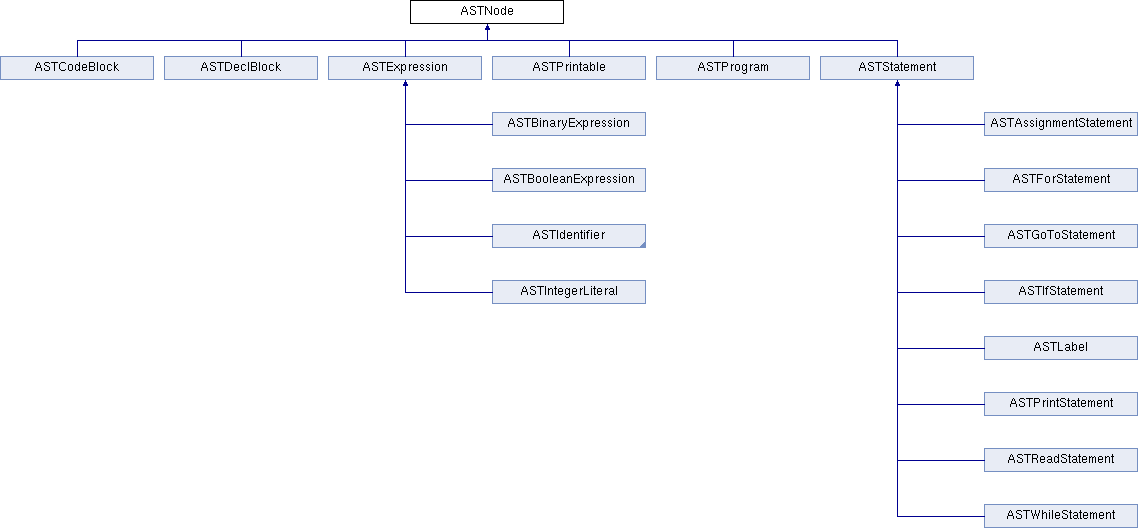
\includegraphics[width=\linewidth]{class_a_s_t_node.png}
  \caption{Inheritance Graph of ASTNode}
  \label{fig:figure1}
\end{figure}
\section*{Visitor Design Pattern}
\addcontentsline{toc}{section}{Visitor Design Pattern}
% \begin{figure}[h]
%  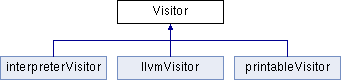
\includegraphics[width=\linewidth]{class_visitor.png}
%  \caption{Inheritance Graph of Visitor}
%  \label{fig:figure2}
% \end{figure}
\section*{Design of Interpreter}
\section*{Design of LLVM Code Generator}
\section*{Performance Comparison}

%-------------------------------------------------------------------------------
% REFERENCES
%-------------------------------------------------------------------------------
% \newpage
% \section*{References}
% \addcontentsline{toc}{section}{References}
% 
% Anand, U., 2010. The Elusive Free Radicals, \textit{The Clinical Chemist,} [e-journal] Available at:<\url{http://www.clinchem.org/content/56/10/1649.full.pdf}> [Accessed 2 November 2013]
% \newline
% \newline
% 
% Biology Forums, 2012. \textit{Normal glomerulus. Acute glomerulonephritis.} [online] Available at: <\url{http://biology-forums.com/index.php?action=gallery;sa=view;id=9284}> [Accessed 23 October 2013].
% \newline
% \newline
% 
% Budisavljevic, M., Hodge, L., Barber, K., Fulmer, J., Durazo-Arvizu, R., Self, S., Kuhlmann, M., Raymond, J. and Greene, E., 2003. Oxidative stress in the pathogenesis of experimental mesangial proliferative glomerulonephritis, \textit{American Journal of Physiology - Renal Physiology,} 285(6), pp. 1138-1148.
% \newline
% \newline
% 
% Chien, C., Lee, P., Chen, C., Ma, M., Lai, M. and Hsu, S., 2001. De Novo Demonstration and Co-localization of Free-Radical Production and Apoptosis Formation in Rat Kidney Subjected to Ischemia/Reperfusion, \textit{Journal of the American Society of Nephrology,} 12(5), pp. 973-982.
% \newline
% \newline
% 
% Couser, W., 1993. Pathogenesis of glomerulonephritis, \textit{Kidney International Supplements,} 42, pp. 19-26.
% \newline
% \newline
% 
% De Gasparo, M., 2002. Angiotensin II and nitric oxide interaction, \textit{Heart Failure Reviews,} [e-journal] Available at:<\url{http://www.ncbi.nlm.nih.gov/pubmed/12379820}> [Accessed 26 October 2013]
% \newline
% \newline
% 
% Edinburgh Renal Education Pages, 2012. \textit{Glomerulonephritis} [online] Available at: <\url{http://www.edrep.org/pages/textbook/glomerulonephritis.php}> [Accessed 25 October 2013].
% \newline
% \newline
% 
% Forbes, J., Coughlan, M. and Cooper, M., 2008. Oxidative Stress as a Major Culprit in Kidney Disease in Diabetes, \textit{Diabetes,} 57(6), pp. 1446-1454.
% \newline
% \newline
% 
% Geeky Medics, 2010. \textit{Glomerulonephritis} [online] Available at: <\url{http://geekymedics.com/2010/10/27/glomerulonephritis/}> [Accessed 25 October 2013].
% \newline
% \newline
% 
% Gryglewski, R., Palmer, R., Moncada, S., 1986. Superoxide anion is involved in the break­down of endothelium derived relaxing factor, \textit{Nature,} 320, pp. 454-456.
% \newline
% \newline
% 
% Halliwell, B., 2001. Free Radicals and other reactive species in Disease, \textit{Encyclopedia of Life Sciences,} [e-journal] Available at:<\url{http://web.sls.hw.ac.uk/teaching/level4/bcm1_2/reading/oxidative_stress/files/Oxidative_stress.pdf}> [Accessed 19 October 2013]
% \newline
% \newline
% 
% Huang, H., Patel, P. and Salahudeen, A., 2001. Lazaroid compounds prevent early but not late stages of oxidant-induced cell injury: potential explanation for the lack of efficacy of lazaroids in clinical trials, \textit{Pharmacological Research,} 41(1), pp. 55-61.
% \newline
% \newline
% 
% Klinger, J., Abman, S. and Gladwin, M., 2013. Nitric Oxide Deficiency and Endothelial Dysfunction in Pulmonary Arterial Hypertension, \textit{American Journal of Respiratory and Critical Care Medicine,} 188(6), pp. 639-646.
% \newline
% \newline
% 
% Lindemann, I., Boettcher, J., Oertel, K., Pasternack, R., Heine, A. and Klebe, G. 2012. Inhibitors of Transglutaminase 2: A therapeutic option in celiac disease, \textit{To be Published,} [e-journal + PDB structure] Available at:<\url{http://www.ebi.ac.uk/pdbe-srv/view/entry/3s3s/summary}> [Accessed 24 October 2013]
% \newline
% \newline
% 
% Mayo Clinic, 2011. \textit{Glomerulonephritis} [online] Available at: <\url{http://www.mayoclinic.com/health/glomerulonephritis/DS00503/}> [Accessed 20 October 2013].
% \newline
% \newline
% 
% McCord, J., Roy, R. and Schaffer, S., 1985. Free radicals and myocardial ischemia. The role of xanthine oxidase, \textit{Advances in myocardiology,} [e-journal] Available at:<\url{http://www.ncbi.nlm.nih.gov/pubmed/2982206}> [Accessed 24 October 2013]
% \newline
% \newline
% 
% National Health Service, 2012. \textit{Causes of glomerulonephritis} [online] Available at: <\url{http://www.nhs.uk/Conditions/Glomerulonephritis/Pages/Causes.aspx}> [Accessed 20 October 2013].
% \newline
% \newline
% 
% Niaudet, P., 2013. \textit{Overview of the pathogenesis and causes of glomerulonephritis in children.} [online] Available at: <\url{http://www.uptodate.com/contents/overview-of- \ the-pathogenesis-and-causes-of-glomerulonephritis-in-children}> [Accessed 21 October 2013].
% \newline
% \newline
% 
% Ronco, P., 2013. \textit{Mechanisms of glomerular crescent formation.} [online] Available at: <\url{http://www.uptodate.com/contents/mechanisms-of-glomerular-crescent-formation}> [Accessed 21 October 2013].
% \newline
% \newline
% 
% Rutchik, J., 2013. \textit{Toxic Neuropathy Clinical Presentation.} [online] Available at: <\url{http://emedicine.medscape.com/article/1175276-clinical#a0216}> [Accessed 26 October 2013].
% \newline
% \newline
% 
% R\&D Systems, 2013. \textit{Technical Information. Ischemia/Reperfusion Injury.} [online] Available at: <\url{http://www.rndsystems.com/cb_detail_objectname_SP96_Ischemia.aspx}> [Accessed 28 October 2013].
% \newline
% \newline
% 
% Salahudeen, A., 1999. Free Radicals in Kidney Disease and Transplantation, \textit{Saudi Journal of Kidney Diseases and Transplantation,} 10(2), pp. 137-143.
% \newline
% \newline
% 
% Sarma, A., Mallick, A. and Ghosh, A., 2010. Free Radicals and Their Role in Different Clinical Conditions: An Overview, \textit{International Journal of Pharma Sciences and Research,} 1(3), pp. 182-192.
% \newline
% \newline
% 
% Shah, S., Baliga, R., Rajapurkar, M. and Fonseca, V., 2007. Oxidants in Chronic Kidney Disease, \textit{Journal of the American Society of Nephrology,} 18(1), pp. 16-28.
% \newline
% \newline
% 
% The University of Utah, Unknown. \textit{Glomerulonephritis} [online] Available at: <\url{http://library.med.utah.edu/WebPath/RENAHTML/RENALIDX.html#8}> [Accessed 25 October 2013].
% \newline
% \newline
% 
% Wang, C. and Salahudeen, A., 1994. Cyclosporine nephrotoxicity: attenuation by an antioxidant -inhibitor of lipid peroxidation in-vitro and in-vivo, \textit{Transplantation,} 58, pp. 940-946.
% \newline
% \newline
% 
% Wang, C. and Salahudeen, A., 1995. Lipid peroxidation accompanies cyclosporine nephrotoxicity: effects of vitamin E, \textit{Kidney International,} 47, pp. 927-934.
% \newline
% \newline
% 
% Weiss, S., 1989. Tissue Destruction by Neutrophils, \textit{New England Journal of Medicine,} 320, pp. 365-376.
% \newline
% \newline


\end{document}

%-------------------------------------------------------------------------------
% SNIPPETS
%-------------------------------------------------------------------------------

%\begin{figure}[!ht]
%	\centering
%	\includegraphics[width=0.8\textwidth]{file_name}
%	\caption{}
%	\centering
%	\label{label:file_name}
%\end{figure}

%\begin{figure}[!ht]
%	\centering
%	\includegraphics[width=0.8\textwidth]{graph}
%	\caption{Blood pressure ranges and associated level of hypertension (American Heart Association, 2013).}
%	\centering
%	\label{label:graph}
%\end{figure}

%\begin{wrapfigure}{r}{0.30\textwidth}
%	\vspace{-40pt}
%	\begin{center}
%		\includegraphics[width=0.29\textwidth]{file_name}
%	\end{center}
%	\vspace{-20pt}
%	\caption{}
%	\label{label:file_name}
%\end{wrapfigure}

%\begin{wrapfigure}{r}{0.45\textwidth}
%	\begin{center}
%		\includegraphics[width=0.29\textwidth]{manometer}
%	\end{center}
%	\caption{Aneroid sphygmomanometer with stethoscope (Medicalexpo, 2012).}
%	\label{label:manometer}
%\end{wrapfigure}

%\begin{table}[!ht]\footnotesize
%	\centering
%	\begin{tabular}{cccccc}
%	\toprule
%	\multicolumn{2}{c} {Pearson's correlation test} & \multicolumn{4}{c} {Independent t-test} \\
%	\midrule	
%	\multicolumn{2}{c} {Gender} & \multicolumn{2}{c} {Activity level} & \multicolumn{2}{c} {Gender} \\
%	\midrule
%	Males & Females & 1st level & 6th level & Males & Females \\
%	\midrule
%	\multicolumn{2}{c} {BMI vs. SP} & \multicolumn{2}{c} {Systolic pressure} & \multicolumn{2}{c} {Systolic Pressure} \\
%	\multicolumn{2}{c} {BMI vs. DP} & \multicolumn{2}{c} {Diastolic pressure} & \multicolumn{2}{c} {Diastolic pressure} \\
%	\multicolumn{2}{c} {BMI vs. MAP} & \multicolumn{2}{c} {MAP} & \multicolumn{2}{c} {MAP} \\
%	\multicolumn{2}{c} {W:H ratio vs. SP} & \multicolumn{2}{c} {BMI} & \multicolumn{2}{c} {BMI} \\
%	\multicolumn{2}{c} {W:H ratio vs. DP} & \multicolumn{2}{c} {W:H ratio} & \multicolumn{2}{c} {W:H ratio} \\
%	\multicolumn{2}{c} {W:H ratio vs. MAP} & \multicolumn{2}{c} {\% Body fat} & \multicolumn{2}{c} {\% Body fat} \\
%	\multicolumn{2}{c} {} & \multicolumn{2}{c} {Height} & \multicolumn{2}{c} {Height} \\
%	\multicolumn{2}{c} {} & \multicolumn{2}{c} {Weight} & \multicolumn{2}{c} {Weight} \\
%	\multicolumn{2}{c} {} & \multicolumn{2}{c} {Heart rate} & \multicolumn{2}{c} {Heart rate} \\
%	\bottomrule
%	\end{tabular}
%	\caption{Parameters that were analysed and related statistical test performed for current study. BMI - body mass index; SP - systolic pressure; DP - diastolic pressure; MAP - mean arterial pressure; W:H ratio - waist to hip ratio.}
%	\label{label:tests}
%\end{table}
